\section{State Space Duality}
\label{sec:ssd}

In \cref{sec:ssm,sec:attention}, we defined structured state space models and structured attention,
discussed their properties, and showed that they both have a quadratic algorithm and a linear algorithm.
This section connects them together.
Our main result is showing that a particular case of structured state space models coincides with a particular case of structured attention,
and that the linear-time SSM algorithm and quadratic-time kernel attention algorithm are dual forms of each other.
\begin{itemize}
  \item \cref{sec:ssd:quadratic-ssm} specializes state space models to scalar structure, where the naive quadratic computation can be seen as an instance of kernel attention.
  \item \cref{sec:ssd:1ss-sma} specializes structured masked attention to semiseparable SMA, which characterizes masked attention with efficient autoregression.
  \item \cref{sec:ssd:ssd} summarizes the connection between structured masked attention and structured state space models, termed structured state space duality.
\end{itemize}

\subsection{Scalar-Identity Structured State Space Models}
\label{sec:ssd:quadratic-ssm}


In \cref{sec:ssm} we showed that state space models are equivalent to semiseparable matrix transformations,
resulting in both a linear recurrent form and quadratic naive form.

Recall that SSMs are defined by $y = \mathsf{SSM}(A, B, C)(x)$, and the matrix form of SSMs uses the SSS (sequentially semiseparable) representation
$M = \mathsf{SSS}(A, B, C)$ where
$M_{ji} = C_j^{\top} A_{j:i} B_i$ (equation \eqref{eq:ssm-matrix}).

Now let us consider the case where $A_j$ is simply a scalar;
in other words, an instantiation of a structured SSM where the $A$ matrices are \emph{extremely} structured: $A = aI$ for scalar $a$ and identity matrix $I$.
Then we can rearrange
\begin{align*}
  M_{ji} = A_{j:i} \cdot (C_j^{\top}B_i)
.
\end{align*}
And this can be vectorized into
\begin{align*}%
  L &\coloneqq \mathsf{1SS}(a) \\
  M &= L \circ (C B^{\top}) \\
\end{align*}
where $B, C \in \R^{\mathtt{(T,N)}}$.

Using this formulation, the full output $Y=MX$ is computed precisely as
\begin{equation}
  \label{eq:ssm-quad}
  \begin{aligned}%
    G     & = \mathsf{contract}(\mathtt{TN, SN \to TS})(C, B) & & \qquad \mathtt{(T,S)} \\
    M     & = \mathsf{contract}(\mathtt{TS, TS \to TS})(G, L) & & \qquad \mathtt{(T,S)} \\
    Y     & = \mathsf{contract}(\mathtt{TS, SP \to TP})(M, X) & & \qquad \mathtt{(T,P)}
  \end{aligned}
\end{equation}
where $\mathtt{S}=\mathtt{T}$.
But this is exactly the same as original definition of masked kernel attention definition \eqref{eq:sha-quad}!

Therefore, as alluded to in \cref{sec:ssm:algorithms},
\emph{naively computing the scalar structured SSM---by materializing the semiseparable matrix $M$ and performing quadratic matrix-vector multiplication---is exactly the same as quadratic masked kernel attention.}

\subsection{1-Semiseparable Structured Masked Attention}
\label{sec:ssd:1ss-sma}

Structured masked attention allows for the use of any structured mask $L$.
When $L$ is the causal mask, it is standard linear attention.
Note that the causal mask is $L = \mathsf{SS}(1_T)$, i.e.\ the $1$-SS mask is generated by $a_t=1$ in definition~\eqref{eq:1ss}.
This motivates generalizing $L$ to the class of 1-semiseparable masks, or \textbf{1-semiseparable structured masked attention (1-SS SMA)},
where the $\mathsf{cumsum}$ in linear attention's recurrence is replaced by a more general recurrence -- the scalar SSM scan, i.e.\ 1-semiseparable matrix multiplication~(\cref{sec:ssm:1-ss}).




Finally, the most important reason we consider 1-semiseparable SMA is because the linear form for computing it is a special case of diagonal state space model.
The linear form of SMA is algorithm \eqref{eq:sha-lin}, where the bottleneck step \eqref{eq:sha-lin:2} can be viewed as matrix multiplication by the 1-SS mask.
In \cref{sec:ssm}, we also wrote out the computation for a diagonal SSM \eqref{eq:ssm-diagonal}, where the bottleneck step \eqref{eq:ssm-diagonal:2} is a scalar SSM recurrence which is equivalent to 1-SS multiplication.
The only difference is that \eqref{eq:ssm-diagonal:2} has an extra $\mathtt{N}$ dimension in $L$, because the matrix $A$ is a diagonal matrix of size $\mathtt{N}$.
This $\mathtt{N}$ dimension would disappear if all diagonal entries of $A$ are the same,
which results in \cref{cor:1ss-sma}.

\begin{corollary}
  \label{cor:1ss-sma}
  1-SS SMA (masked attention with 1-semiseparable structured matrices $L$)~\eqref{eq:sha-lin} is a special case of a diagonal SSM~\eqref{eq:ssm-diagonal} where the diagonal matrix is a scalar multiple of the identity.
\end{corollary}

While \cref{cor:1ss-sma} says that 1-SS SMA has an efficient recurrent form,
we can also show a converse result that characterizes which instances of SMA has efficient autoregression.
\begin{theorem}
  \label{thm:ss-sma}
  For any instantiation of structured masked attention (\cref{def:sma}) that is an autoregressive process with bounded order,
  the structured mask $L$ must be a semiseparable matrix.
\end{theorem}
In other words, efficient autoregressive attention is general \emph{semiseparable SMA}.
\cref{thm:ss-sma} is proved in \cref{sec:theory-details:ssm-sma}.

\begin{remark}
  While 1-semiseparable SMA is a special case of a state space model,
  general semiseparable SMA is strictly more expressive than 1-SS SMA, and cannot be described by a standard SSM.
  However, the semiseparable multiplication by $L$ and the linear form of SMA (equation \eqref{eq:sha-lin:1}) each involve an expansion and contraction step, and can be absorbed into a similar instance of 1-SS SMA with a single (larger) expansion.
\end{remark}


In summary, 1-semiseparable structured attention is the most important case of SMA, because it is:
\begin{itemize}
  \item a natural generalization of linear attention with an input-dependent recurrence.
  \item the simplest case of general semiseparable attention, which is equivalent to efficient autoregressive attention.
  \item a special case of a diagonal state space model.
\end{itemize}

\subsection{Structured State-Space Duality (SSD)}
\label{sec:ssd:ssd}

To summarize our results:
\begin{itemize}
  \item Structured state-space models (\cref{sec:ssm}) are a model usually defined through a linear-time recurrence.
    However, by expanding the matrix formulation characterizing its linear sequence-to-sequence transformation, one can derive a quadratic form.
  \item Attention variants (\cref{sec:attention}) are a model defined through quadratic-time pairwise interactions. However, by viewing it as a four-way tensor contraction and reducing in a different order, one can derive a linear form.
  \item A natural special case of each one -- 
    more precisely, state space models with scalar-identity structure on the $A$ matrices, and structured masked attention with 1-semiseparable structure on its $L$ mask
    -- are duals of each other with the exact same linear and quadratic forms.
\end{itemize}
\cref{fig:ssd} summarizes the duality between these two representations.




\begin{figure*}
  \begin{minipage}[c]{.49\linewidth}
    \small
    \centering
    \begin{tabular}{@{}lll@{}}
      \toprule
      Structured State Space Model                                  & Structured Masked Attention                               \\
      \midrule
      $C$ \hfill (contraction matrix)                                    & $Q$ \hfill (queries)                                      \\
      $B$ \hfill (expansion matrix)                                     & $K$ \hfill (keys)                                         \\
      $X$ \hfill (input sequence)                                   & $V$ \hfill (values)                                       \\
      $A_{j:i}$ \hfill (state matrix)                               & $L_{ji}$ \hfill (mask)                                    \\
      $\mathtt{N}$ \hfill (state expansion dim.)                    & $\mathtt{N}$ \hfill (kernel feature dim.)              \\
                                                                    \midrule
      $H$ \hfill (hidden states \eqref{eq:ssm-diagonal:2})          & \qquad \multirow{2}{*}{SMA linear dual \eqref{eq:sha-lin}} \\
      $\quad = L \cdot XB$ \hfill (linear mode)                     &                                                          \\
      \midrule
      \qquad \multirow{2}{*}{SSM quadratic dual \eqref{eq:ssm-quad}} & $G$ \hfill (Gram matrix \eqref{eq:sha-quad:1})            \\
                                                                    & $\quad = Q \cdot K^{\top}$ \hfill (quadratic mode)        \\
      \bottomrule
    \end{tabular}
  \end{minipage}
  \hfill
  \begin{minipage}[c]{0.49\linewidth}
    \centering
    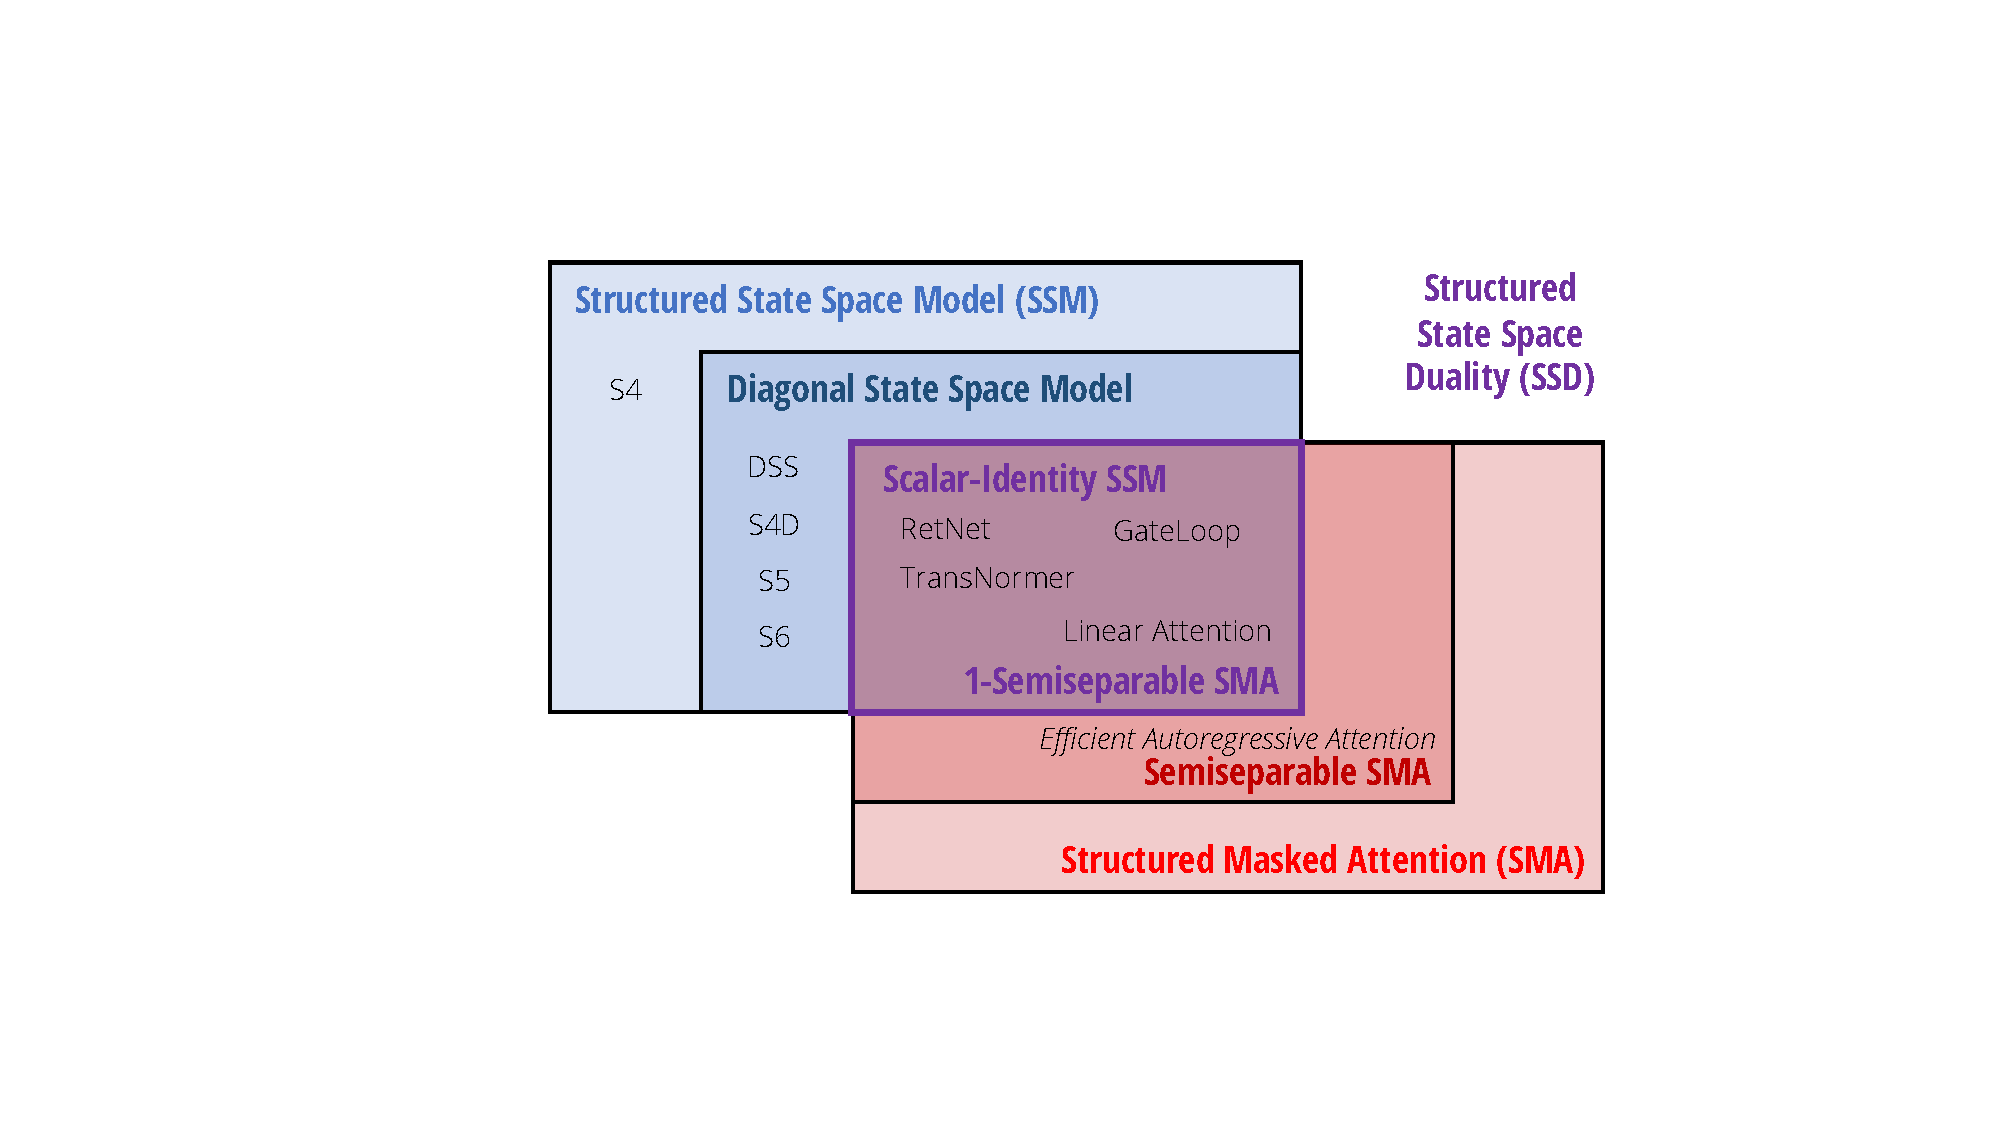
\includegraphics[width=\linewidth]{fig/ssd_venn.pdf}
  \end{minipage}
  \captionsetup{type=figure}
  \caption{
    (\textbf{Structured State Space Duality}.)
    State space duality describes the close relationship between state space models and masked attention.
    (\emph{Left}) General SSMs and SMA both possess linear and quadratic forms, with direct analogs in notation.
    (\emph{Right}) SSMs and SMA intersect at a large class of \emph{state space dual models} (SSD) which capture many sequence models as special cases.
  }
  \label{fig:ssd}
\end{figure*}

An extended related work and discussion (\cref{sec:related}) describes the relationship between SSD and general SSMs / attention in more detail.


